\documentclass[tikz,border=7pt]{standalone}
\usepackage[T1]{fontenc}
\usepackage{lmodern}
\usetikzlibrary{arrows.meta,positioning,shapes.geometric,fit,backgrounds,calc}
\begin{document}
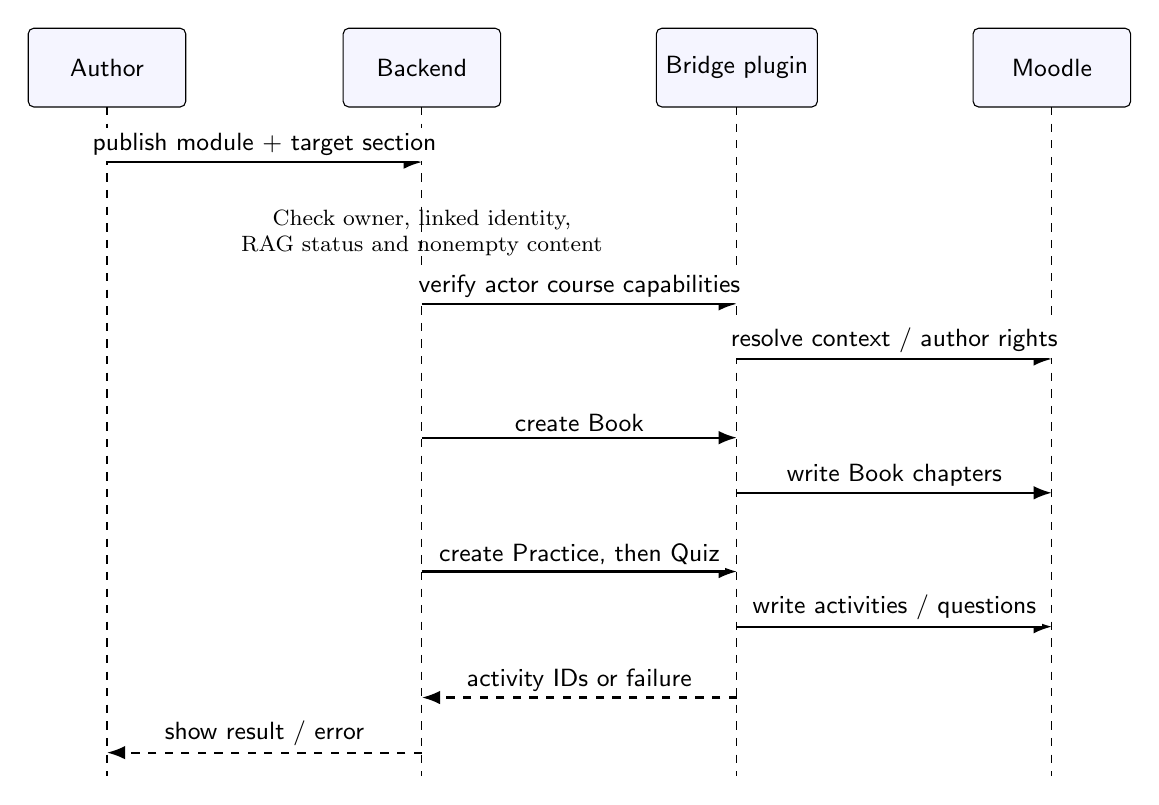
\begin{tikzpicture}[font=\sffamily\small,>=Latex,
box/.style={draw,rounded corners=2pt,align=center,minimum width=3cm,minimum height=1cm,fill=blue!4},
entity/.style={draw,rectangle,align=center,minimum width=2.6cm,minimum height=.75cm,fill=blue!4},
rel/.style={draw,diamond,aspect=2,inner sep=2pt,align=center,font=\sffamily\footnotesize,fill=yellow!8},
attr/.style={draw,ellipse,inner sep=3pt,font=\sffamily\footnotesize},
uc/.style={draw,ellipse,align=center,minimum width=4cm,minimum height=.9cm},
flow/.style={->,thick},lab/.style={font=\sffamily\small,fill=white,inner sep=2pt}]

\foreach \n/\x/\label in {t/0/Author,b/4/Backend,p/8/Bridge plugin,m/12/Moodle} {
\node[box,minimum width=2cm] (\n) at (\x,0) {\label};
\draw[dashed] (\x,-.5) -- (\x,-9);
}
\draw[flow] (0,-1.2) -- node[lab,above]{publish module + target section} (4,-1.2);
\node[align=center,font=\footnotesize] at (4,-2.1) {Check owner, linked identity,\\RAG status and nonempty content};
\draw[flow] (4,-3) -- node[lab,above]{verify actor course capabilities} (8,-3);
\draw[flow] (8,-3.7) -- node[lab,above]{resolve context / author rights} (12,-3.7);
\draw[flow] (4,-4.7) -- node[lab,above]{create Book} (8,-4.7);
\draw[flow] (8,-5.4) -- node[lab,above]{write Book chapters} (12,-5.4);
\draw[flow] (4,-6.4) -- node[lab,above]{create Practice, then Quiz} (8,-6.4);
\draw[flow] (8,-7.1) -- node[lab,above]{write activities / questions} (12,-7.1);
\draw[flow,dashed] (8,-8) -- node[lab,above]{activity IDs or failure} (4,-8);
\draw[flow,dashed] (4,-8.7) -- node[lab,above]{show result / error} (0,-8.7);
\end{tikzpicture}
\end{document}
